\documentclass{article} % For LaTeX2e
\usepackage{nips13submit_e,times}
\usepackage{hyperref}
\usepackage{url}
\usepackage{graphicx}
\usepackage{amsmath}
\usepackage{amssymb}
%\documentstyle[nips13submit_09,times,art10]{article} % For LaTeX 2.09


\title{  Extracting Aspect-Level Sentiment from Product Reviews  }


\author{
Desmond C. Ong, Shane Soh, Matthew Long \\
Stanford University \\
\texttt{\{dco, shanesoh, mlong14\}@stanford.edu}
%Matthew Long \\
%Stanford University\\
%\texttt{mlong14} \\
%\And
%Desmond C. Ong \\
%%Psychology \\
%Stanford University \\
%\texttt{dco} \\
%\And
%Shane Soh \\
%%Affiliation \\
%Stanford University \\
%\texttt{shanesoh} \\
}

% The \author macro works with any number of authors. There are two commands
% used to separate the names and addresses of multiple authors: \And and \AND.
%
% Using \And between authors leaves it to \LaTeX{} to determine where to break
% the lines. Using \AND forces a linebreak at that point. So, if \LaTeX{}
% puts 3 of 4 authors names on the first line, and the last on the second
% line, try using \AND instead of \And before the third author name.

\newcommand{\fix}{\marginpar{FIX}}
\newcommand{\new}{\marginpar{NEW}}

\nipsfinalcopy % Uncomment for camera-ready version

\begin{document}


\maketitle

\begin{abstract}
Previous work in \textit{aspect-level sentiment analysis}---identifying the sentiment associated with various attributes of a product---have mostly been formulated as supervised learning problems, requiring labels of both the relevant aspects and their sentiment. Acquiring labels for sufficiently large datasets are however often costly and time consuming. Here we propose a largely unsupervised and scalable method for aspect-level sentiment analysis that consists of two steps: 1) discovery and extraction of aspects from product reviews via clustering of \texttt{word2vec} representations, 2) classifying aspect-specific sentiments using convolutional neural networks.
\end{abstract}

\section{Introduction}


In this day and age, consumers have unprecedented access to a deluge of information about products---most notably, reviews written by other consumers---with which to make his or her purchase decisions. Unfortunately, sifting through hundreds of reviews across tens of different websites to acquire specific information about the product and its important attributes (e.g. \textit{battery life}, \textit{screen size}, or \textit{weight} in the case of electronic products) is a time-consuming chore. Fortunately, the proliferation of customer reviews on websites such as Amazon.com has made it possible, with the right tools, to leverage the ``wisdom of the crowd" when making purchase decisions. Aspect-level sentiment analysis would allow consumers to effortlessly compare relatively unbiased sentiments of various aspects of multiple similar products.

However, one of the biggest challenges in training aspect-specific sentiment analysis models is the lack of large datasets labeled with sentiment on the aspect-level (for most datasets, sentiment labels exist on a document level). In this report, we propose a scalable and efficient method for extracting and classifying aspect-specific sentiments that is largely unsupervised. To do this, we tackle two separate but interconnected components of this problem: 1) discovery of aspects, and 2) aspect-specific sentiment classification.

Within the context of a product review, the first component, \textit{aspect discovery}, involves identifying individual ``aspects" (which could be the product itself, or features/attributes of the product). This is made more difficult by the fact that relevant aspects might differ greatly across products in the same category. For example, aspects revelant to a cellular phone might be \textit{battery life}, \textit{screen size}, \textit{weight} and \textit{cost}. Not all these aspects are relevant across electronic items: for instance, \textit{screen size} might be irrelevant for a pair of headphones or a video game controller. We tackle this problem by generating new aspects from a list of seed words based on cosine similarities of the \texttt{word2vec} representations [1-2], and using the discovered aspects to train an aspect classifier.

The second component, \textit{aspect-specific sentiment classification} involves identifying the sentiment associated with each aspect [3-8]---\textit{very positive, positive neutral, negative or very negative}. We approach this problem by first using a lexicon-based heuristic as a baseline and as a means of \textit{pre-labeling} the data. We then refined the labels and trained a convolutional neural network [10] to tackle the sentiment analysis problem as a sentence classification problem.

\section{Related work}


\textbf{Aspect Discovery}: Previous methods have used graphical models to attempt to extract latent sentiment. [3-5] use variants of Latent Dirichlet Allocation to model latent aspects. In particular, these methods have a generative model where there is a latent aspect drawn from a mix of ``global" and ``local" topics [3-4], latent to each sentence [5].

% Add in "Simpler is better" paper

% [aspect parser paper]: rule-based approach to extracting aspects

\textbf{Aspect-specific Sentiment Classification}: [3,5] add sentiment into their generative model of aspects and infer the sentiment using Gibbs sampling. [4,6] use heuristics to match the sentiment to aspects. Other deep learning approaches for aspect-based sentiment analysis use hierarchical models such as a Recursive Neural Tensor Network (RNTN) to extract aspect-sentiment tuples [7-9]. Unfortunately, such supervised methods that require labeled aspects-sentiment pairs for training are unscalable, and a better approach would be to automatically identify relevant aspects for each product (which, e.g. [3-5] try to do via topic modeling). More recently, there has been work on using convolutional neural networks (CNN) trained on top of pre-trained word vectors for sentence-level classification tasks [10]. Specifically, [10] demonstrated the use of CNN to outperform state-of-the-art models on sentiment analysis classification tasks.

% TODO: Desmond to add more references?

\section{Dataset}
The dataset that we used consists of 7.6 million reviews (39.4M sentences) of electronic products from Amazon.com [11]. Each review is labeled with the document-level 5 star rating, which we did not end up using as it was too coarse. We focused our attention on the raw natural language text. We additionally supplemented our dataset with reviews for more recent products.

\textbf{Preprocessing.} We tokenized our corpus using NLTK's punkt tokenizer [12] for sentence splitting. We then removed all non-alphanumerical characters and replaced all digits with \texttt{DG}. Finally, we performed collocation detection to detect common bigrams.

\section{Approach}

Our proposed workflow can be broadly divided into two main parts: {\bf Aspect Discovery} and {\bf Aspect-Specific Sentiment Classification}. See Fig. \ref{workflow} for an illustration.

\begin{figure}[ht]
\begin{center}
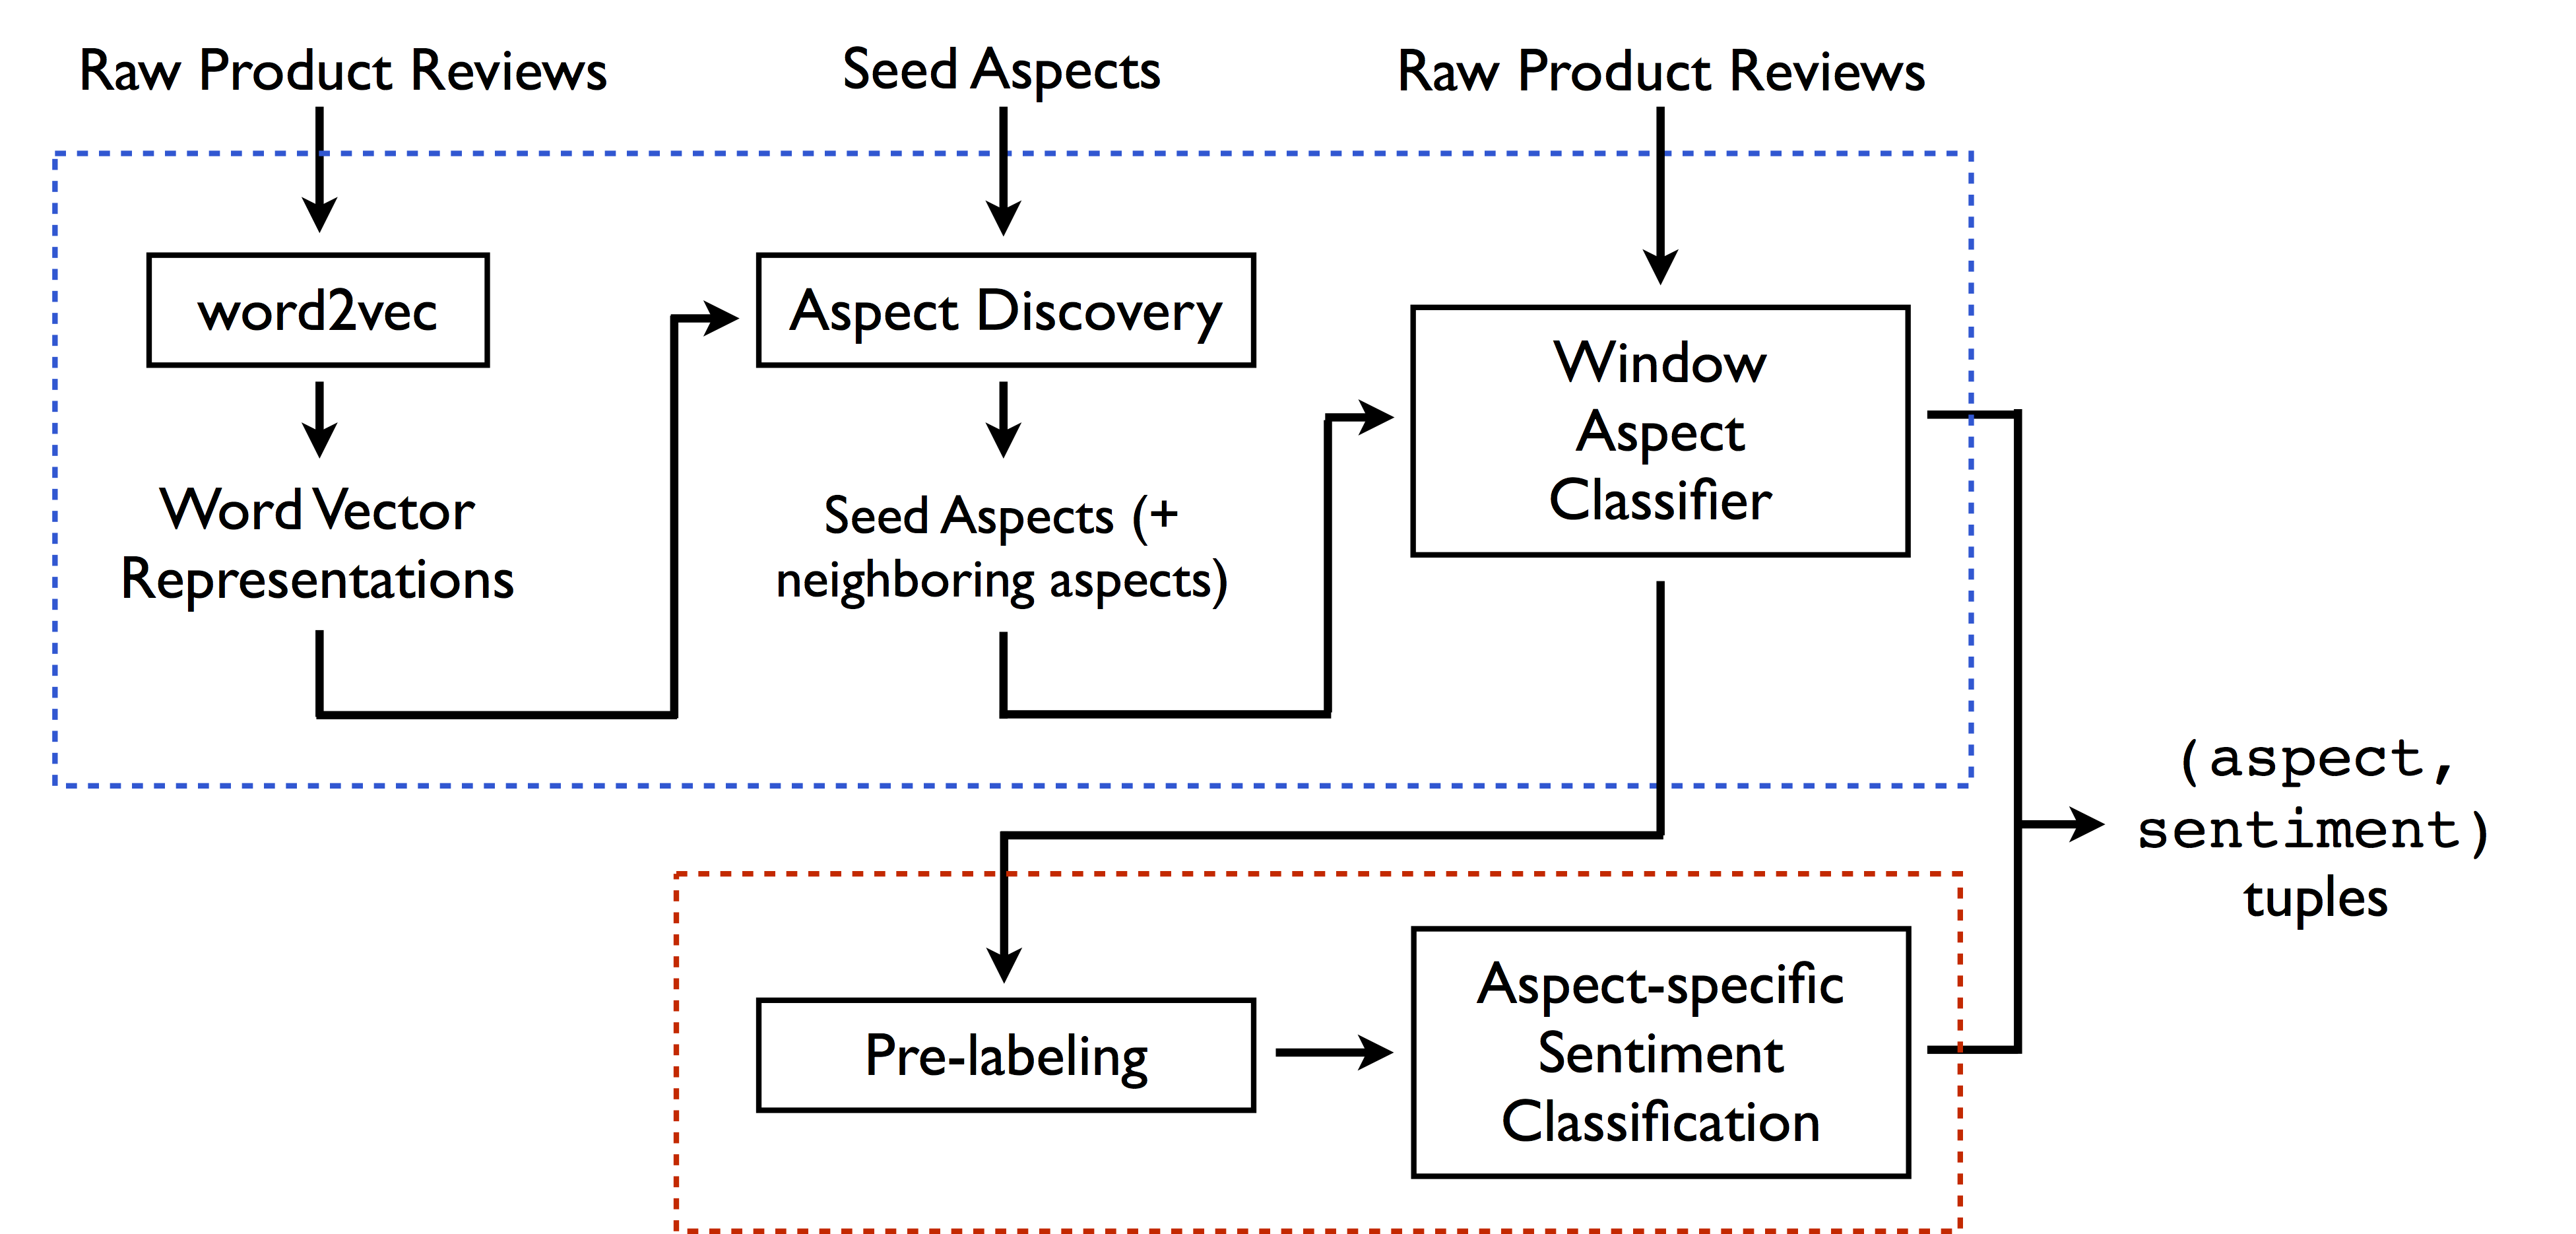
\includegraphics[width=.85\columnwidth]{workflow.png}
\end{center}
\caption{Proposed Workflow. We generate a list of seed aspects specific to the product category. We then discover neighboring aspects based on cosine distances to the seed aspects' \texttt{word2vec} representations. We then train a \textit{window aspect classifier} to discover more aspects from raw text. Next, we use a lexicon-based heuristic to \textit{pre-label} the expanded list of aspects which are subsequently refined by hand. Lastly, we train a supervised CNN to do the \textit{aspect-specific sentiment classification} to produce \texttt{(aspect, sentiment)} tuples.}
\label{workflow}
\end{figure}

\subsection{Aspect Discovery}
The first half of our workflow involves discovering a list of aspects specific to the products in a particular product category given a list of seed aspects.

\textbf{Generating Seed Aspects}. This step involves generating a list of seed aspects. These seed aspects do not require domain-specific knowledge and can be fairly general (the idea is that any layperson should be able to generate these words about most product categories). In our case, we generated 56 seed aspects specific to electronic products such as \textit{screen quality, construction, durability, cost}. 

\textbf{Aspect Discovery}. To generate aspects in an unsupervised fashion, we trained a \texttt{word2vec} model on our dataset and discovered neighboring aspects based on cosine distances to the seed aspects' word vector representations. Our intuition is that we can use similarities in a high dimensional word vector embedding space to find closely related groups of words. Words may be grouped by syntactic class (e.g. nouns), by similarity in context (e.g. ``X is great"), or by other words that they co-occur with.

\textbf{Window Aspect Classifier}. We used the output from the aspect discovery process as labels to train a sliding window-based aspect classifier. This allows us to run the classifier on the raw review text to extract more aspects that we might have missed out in the discovery process, or to extract aspects from other product categories.

There are two classes: \texttt{ASP} for aspects and \texttt{O} for words that are not aspects.

This model is a 2-layer neural network where the input is a window consisting of a word concantenated with its immediate neighbors. In this case of a window of size 3, the input is
\begin{align}
x^{(t)} = [ L x_{t-1}, L x_t, L x_{t+1} ] \in \mathbb{R}^{3d}
\end{align}
where $x_{t-1}, x_t, x_{t+1}$ are one-hot vectors into a word-representation matrix $L \in \mathbb{R}^{d \times \vert V \vert}$, where d is the \texttt{word2vec} dimensions and $\vert V \vert$ is the number of words in the vocabulary. We compute our predictions as:
\begin{align}
h &= tanh(W x^{(t)} + b_1)\\
\hat{y} &= softmax (Uh + b_2)\\
J(\theta) &= -\sum_{k=1}^{2} y_k \log \hat{y}_k
\end{align}

where $y \in \mathbb{R}^2$ is a one-hot label vector. When computing the loss for the training set, we average $J(\theta)$ with respect to each training example.

\subsection{Aspect-Specific Sentiment Classification}
The second half of our workflow involved sentiment analysis given identified aspects. Our intuition for this part stems from locality: if there are multiple sentiment and multiple aspect words within a sentence, then a good intuition would be that sentiment words closer to a particular aspect should be attributed to that aspect. Hence, models should be able to make use of local context to help in attributing sentiment.

\textbf{Pre-labeling using Lexicon-based Heuristic}.
Using the expanded list of aspects (from the aspect discovery process), we label them using a heuristic based on a sentiment lexicon by Hu and Liu [13]. We obtained phrases (i.e. training examples) consisting of an identified aspect in the middle, surrounded by a context window of $m$ words on both sides. We also padded these phrases with sentence start and end tags and zero-padded them to a fixed length. Next, we labeled all unigrams in these phrases with their unigram-specific sentiment according to the lexicon by [13] and averaged them to obtain the label for each phrase. Having pre-labeled our phrases according to this heuristic, we were then better able to refine the labels manually in less time (and hence less cost).


\begin{figure}[ht]
\begin{center}
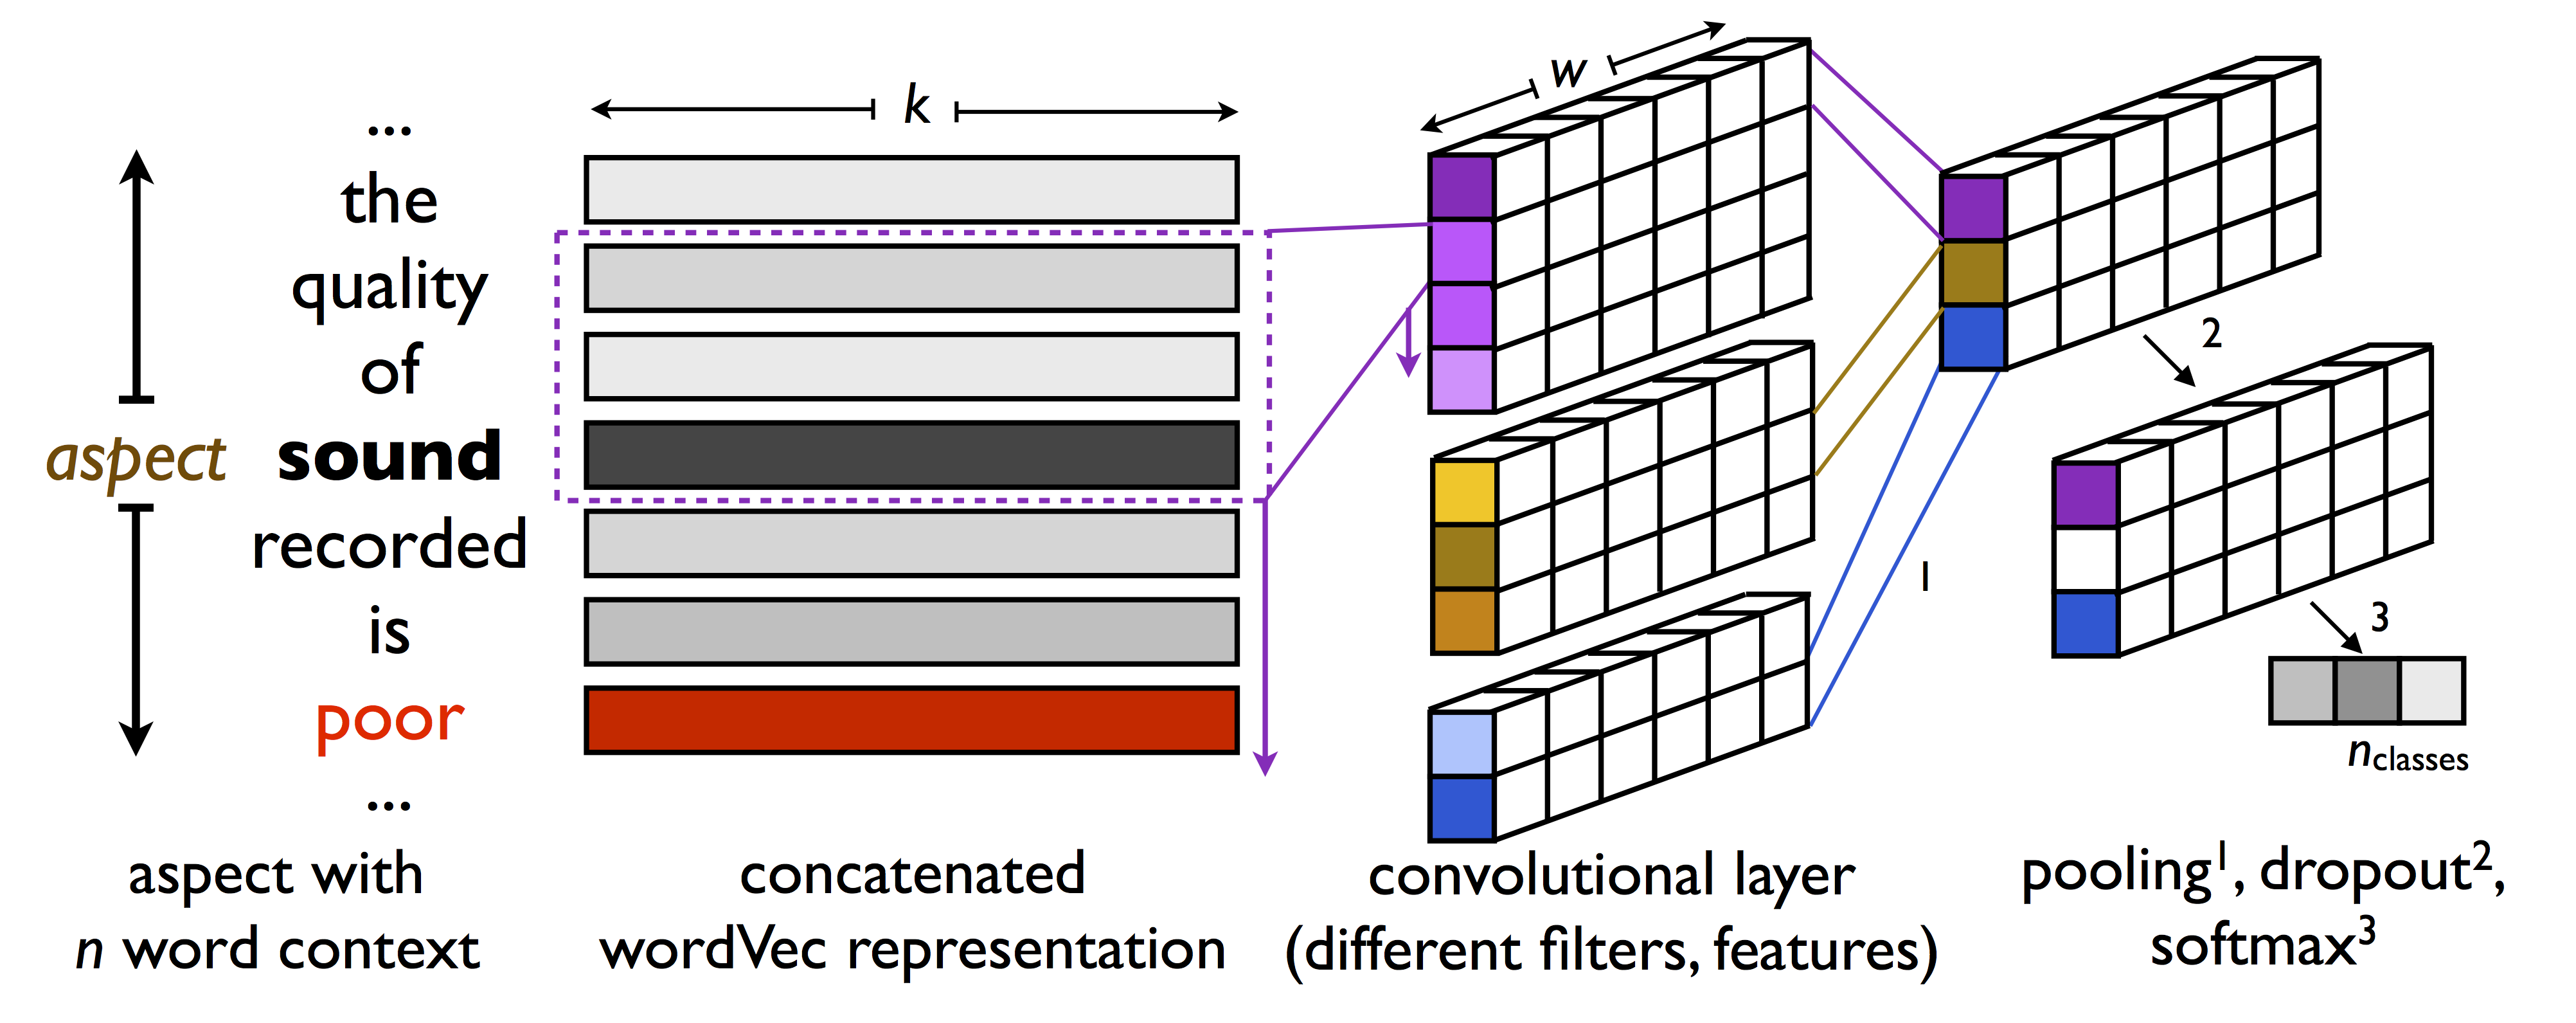
\includegraphics[width=\columnwidth]{model_architecture.png}
\end{center}
\caption{CNN Model Architecture as documented by Kim [10]. The input is an $2m+1$ word context, where $m$ is the number of words on each side of the aspect, and the center word is an identified aspect. The input is convolved with different filter sizes with $w$ features and is then max-pooled.}
\label{architecture}
\end{figure}

\textbf{Sentiment Classification}. We decided upon a Convolutional Neural Network (CNN) Model based after Kim [10], who reported excellent results in sentence classification on many tasks including sentiment analysis. We model our architecture as per [10] and as reproduced in Figure \ref{architecture}. This model has one convolutional layer trained on top of pre-trained word vectors obtained from a \texttt{word2vec} model trained on our dataset. However, unlike [10], our CNN uses only a single non-static channel which allows the word vectors to be further finetuned.

Our input is represented as:
\begin{align}
	x_{1:2m+1} = x_1 \oplus x_2 \oplus \ldots \oplus x_{m+1} \oplus \ldots \oplus x_{2m+1}
\end{align}
where $\oplus$ is the concatenation operator, $n$ is the sentence length, $x_i \in \mathbb{R}^k$ is a k-dimensional word vector of the i-th word, and $x_{m+1}$ is the aspect word. Convolution using multiple filters $w \in \mathbb{R}^{hk}$ of various sizes $h$ is applied to the input to produce new features. A feature $c_i$ is generated from a window of words $x_{i:i+h-1}$ as such:
\begin{align}
c_i = ReLU(\textbf{w} \cdot \textbf{x}_{i:i+h-1} + b)
\end{align}
This filter is applied across the input phrase to produce a feature map $\textbf{c} = [c_1, c_2, \ldots, c_{n-h+1}] \in \mathbb{R}^(n-h+1)$. We then apply a max-over-time pooling operation over each feature map and retain the maximum value $\hat{c} = max \{\textbf{c}\}$ for each filter.

Lastly, we employ dropout [14] in the fully connected layer and take the softmax output to obtain the predictions for all five sentiment classes.


\section{Experimental Results} 

\subsection{Aspect Discovery} 

\subsubsection{word2vec Model}
\begin{figure}[ht]
\begin{center}
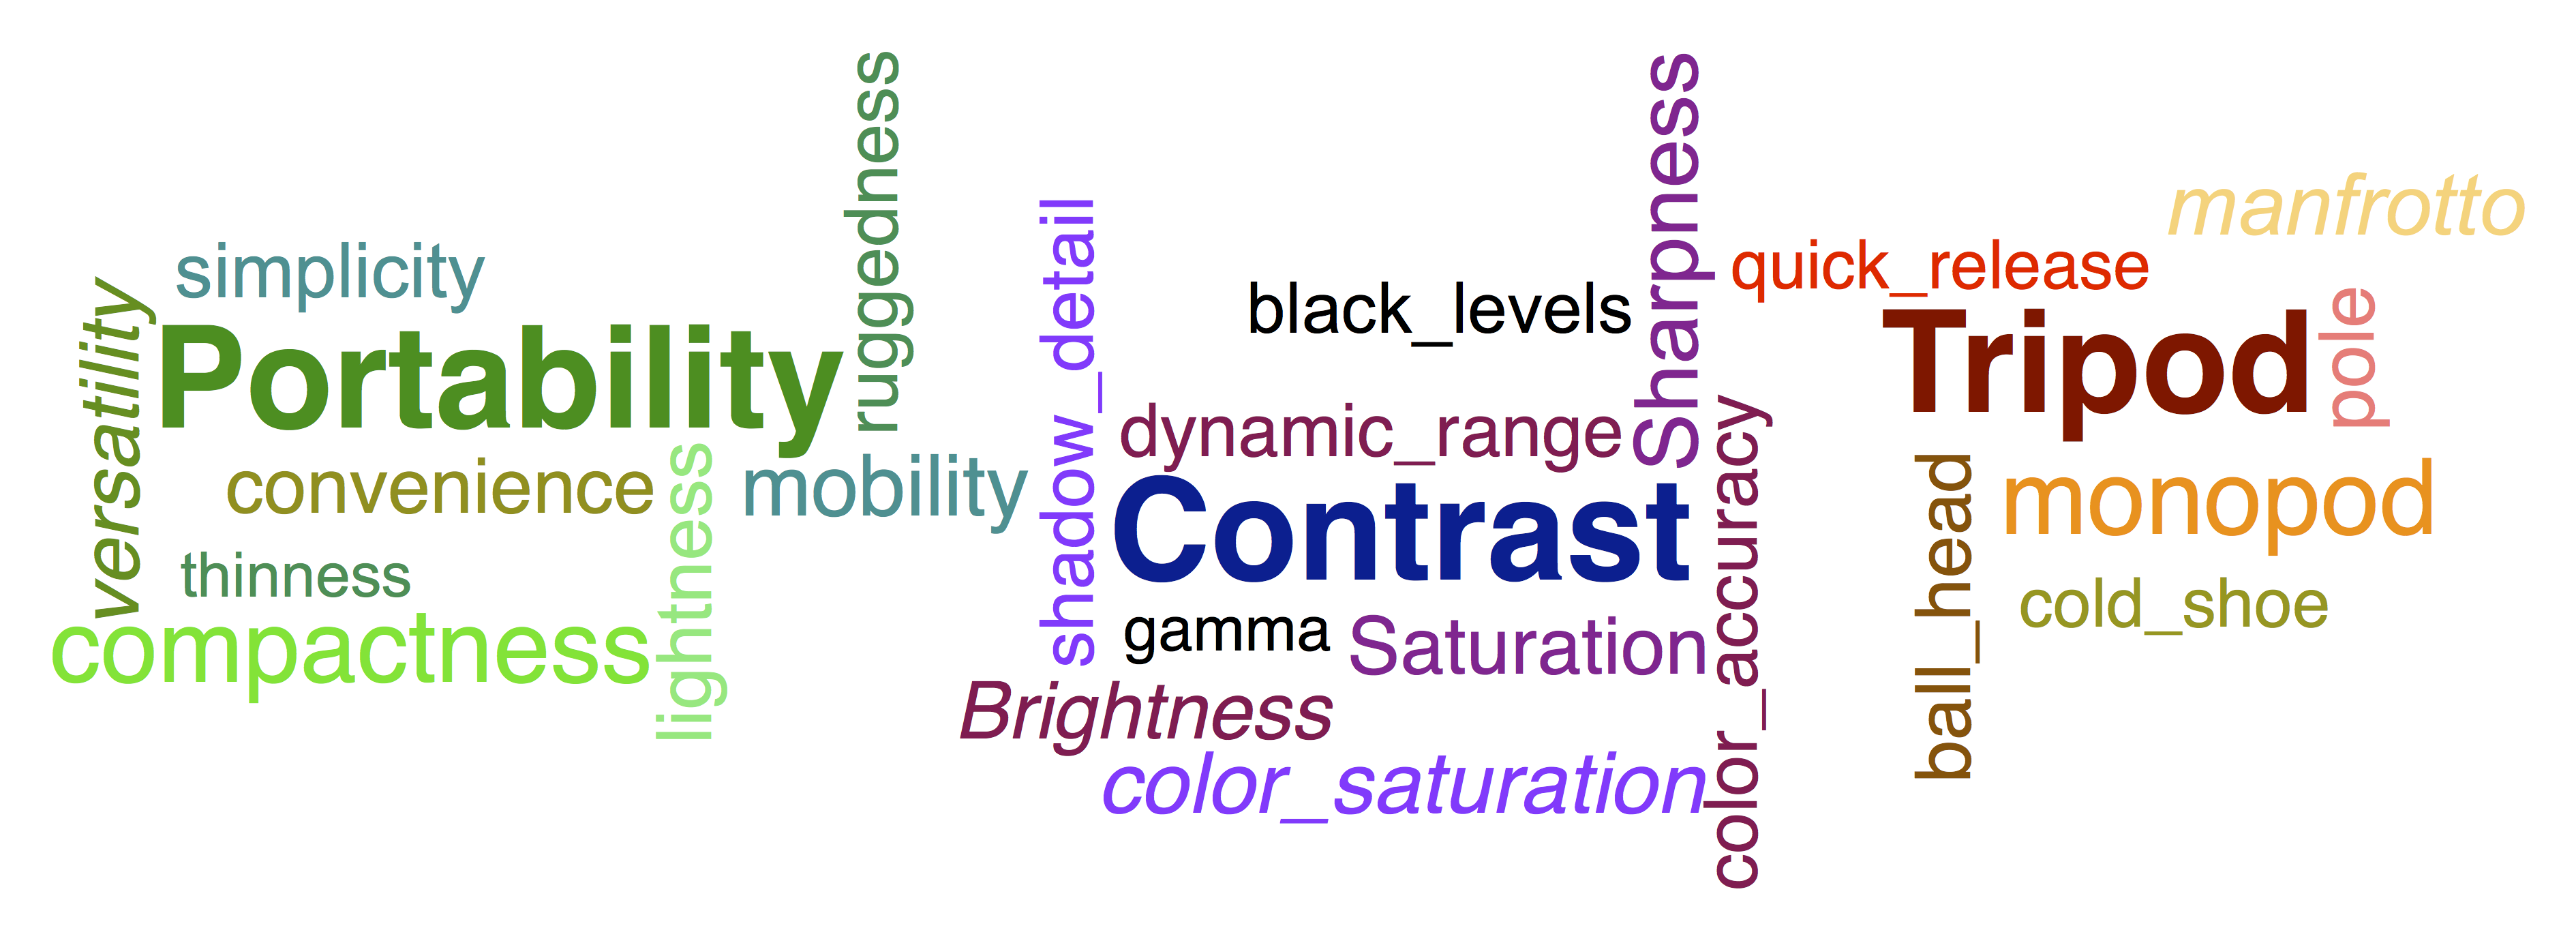
\includegraphics[width=\columnwidth]{Aspects_long.png}
\end{center}
\caption{Aspects Discovery. Word clouds generated by seeding \texttt{portability} (left), \texttt{contrast} (middle), and \texttt{tripod} (right). Words are sized according to cosine similarity with the seed word.}
\label{aspectFig}
\end{figure}

We trained three different \texttt{word2vec} models. The most successful model was trained using the CBOW (continuous bag-of-words) model with a window size of 10 and feature dimension size of 300. We also ignored all words with total frequency count below 40 (this helped to remove many misspellings and typos). We determined the performance of each model by querying the model with various aspects common to electronic products (e.g. ``portability", ``screen quality", etc) and returning the top-$n$ closest attributes based on cosine similarity. We also found that training our own \texttt{word2vec} model is essential for good performance in this case as many of our vocabulary contain very niche words specific to electronic products (e.g. ``gold\_plated", ``atx\_motherboard", ``sli").

Figure \ref{aspectFig} illustrates the top-$n$ closest results for the seed words \texttt{portability}, \texttt{contrast}, and \texttt{tripod}. After qualitative evaluation, we found that an $n$ of 5 is a good number that maintains the quality of aspects while allowing for good discovery.

As shown in Fig. \ref{aspectFig}, words like \texttt{portability} returned many synonyms as well as product aspects that are related to it (e.g. \texttt{ruggedness} and \texttt{simplicity}). Our model is also capable of returning aspects that are specific and unique to the product category it is trained on. In this case of electronic products, a query like \texttt{contrast} returned words like \texttt{shadow\_detail}, \texttt{dynamic\_range}, \texttt{black\_levels} and \texttt{gamma}, which are aspects specific to devices like monitor displays and cameras. Finally, the query \texttt{tripod} returned various aspects of camera tripods, many of them being features that are non-obvious to the layperson. For instance, \texttt{ball\_head} refers to a type of ball-shaped tripod head that allows free-pivoting along two rotational axes (as opposed to Cartesian axes), and \texttt{quick\_release} refers to tripod mounts that come with a quick-release plate. Many of these queries would otherwise perform poorly if performed on lexical databases like WordNet.

We also found that out of 336 discovered aspects (56*5 neighboring aspects + 56 seed aspects), only 9 words are considered to be non-aspect words, giving us an accuracy of \textbf{97.32\%}. We also found that the aspect discovery process was useful in discovering unintuitive but highly related words such as acronyms (e.g. \texttt{ui} and \texttt{gui}, \texttt{kb} and \texttt{keyboard}), common typos (e.g. \texttt{qaulity}, \texttt{quaility}) and synonymous words (e.g. \texttt{trackpad}, \texttt{touchpad}).

\subsubsection{Window Aspect Classifier}
We performed hyperparameter tuning on our window classifier and found that window of size 5, regularization strength of 0.001 and learning rate of 0.01 using a minibatch schedule produced the best performing model. This was trained on a randomly sampled subset of 20,000 sentences, each of which containing at least one aspect. The training dataset consists of 48,368 \texttt{ASP}-labeled words and 848,218 \texttt{O}-labeled words. 

As our dataset is heavily unbalanced (towards having 95\% positive \texttt{ASP} examples), we evaluate our window aspect classifier primarily by its ability to recall positive example (i.e. intuitively the ability of the classifier to find all the aspects). In this case, our best performing classifier has an \texttt{ASP} recall of \textbf{92.45\%} and a precision of \textbf{99.15\%}, i.e. it is capable of finding 92.45\% of the aspects and practically did not mislabel any non-aspect words as aspects.

\subsection{Aspect-specific Sentiment Classification}

\begin{table}[t]
\begin{center}
\begin{tabular}{lll}
\multicolumn{1}{c}{\bf Aspect Detection Model}  &\multicolumn{1}{c}{\bf Recall}  &\multicolumn{1}{c}{\bf Precision} \\ \hline
Sliding Window Classifier & 92.45\%  & 99.15\%\\
&\\
\end{tabular}
\begin{tabular}{lll}
\multicolumn{1}{c}{\bf Sentiment Model}  &\multicolumn{1}{c}{\bf 3-class Accuracy} &\multicolumn{1}{c}{\bf 5-class Accuracy} \\ \hline
 Convolutional Neural Network \textsuperscript{1} & 79.63\% & 64.78\% \\
 Pre-trained out-of-domain RNTN [9]\textsuperscript{2}       & 51.1\% & 42.3\% \\
 Lexicon-based heuristic	& 75.25\% & -- \\
\end{tabular}
\end{center}
\caption{Performance of different models. Top: Recall of the RNN in our aspect detection model. Bottom: Accuracies on the sentiment analysis task. \textsuperscript{1} is described in Fig. \ref{architecture} and was trained in domain, while \textsuperscript{2} is an RNTN pre-trained on movie review data. The interpretation is discussed more in text.}
\label{ModelResultsTable}
\end{table}

\subsubsection{Pre-labeling}
Using the aforementioned steps, we obtained the 6,000 labeled examples which consisted of an identified aspect in the middle, surrounded by a context window of 5 words on both sides. We padded these phrases with sentence start and end tags and zero vectors. Next, we manually re-labeled these 6,000 examples on a 5 point scale, corresponding to \textit{very negative, negative, neutral, positive, and very positive}.

Our lexicon-based heuristic has a \textbf{75.25\%} classification accuracy with 3 classes, i.e. only 24.75\% of the 6,000 examples has to be re-labeled into 5 classes. This pre-labeling greatly sped up our labeling process to approximately 8 man-hours for all 6,000 examples. This heuristic also provides us with a baseline accuracy for our CNN sentence classification model.

Our labeled dataset of 6,000 examples is comparable to existing available aspect-sentiment datasets (e.g. the Beer Advocate dataset and Camera Review dataset reported in [8] had 8,000 and 4,000 labeled examples respectively).

% Socher's model (down the rows) vs. human labels. So there were 16 instances that human says 2 and model says 1.
%							True Labels
%			1		2		3		4		5
%1			9		16		5		10		4		44
%2			168		495		404		180		124		1371
%3			230		590		1528		488		303		3139
%4			21		70		494		490		281		1356
%5			0		0		9		65		16		90
%			428		1171		2440		1233		728		6000

\subsubsection{Convolutional Neural Network Sentiment Classifier}
We trained our CNN on using the 6,000 labeled examples and evaluated using 10-fold cross validation. The results are given in Table \ref{ModelResultsTable}. The CNN, with 3 filters of size 3, 4 and 5 and hidden layer dimensions of 300 achieved an accuracy of \textbf{64.78\%} on the 5-class (\textit{very positve, positive, neutral, negative, very negative}) classification, and \textbf{79.63\%} on the coarser 3-class (\textit{positve, neutral, negative}) classification task.

We also considered the possibility of using existing pre-trained sentiment classification models to test on the discovered aspect (as opposed to training a sentiment classifier as we did). For instance, there are recursive neural network models (e.g. Socher et al [9]) that are trained on larger and more granular labeled data. However, these models are often trained on other domains ([9] was trained on movie reviews) and it is still an open question as to the degree of cross-domain generalization. To test this, we ran the model (as implemented in Stanford CoreNLP Sentiment Analysis [9]) on our 6,000 labeled examples. The 5-class accuracy was 42.3\%, while the 3 class accuracy was 51.1\%.

The difference in accuracy was largely a result of testing the model out of domain (while our model was trained within domain). In particular, there are words that most likely do not exist in the vocabulary of [9] (e.g. words like "motherboard" and "pixel\_density"). We note, however, that [9] reported a test accuracy on their own dataset of 45.7\% on a 5-class task---a performance that is comparable to what we found.

\subsection{Qualitative Evaluation of Overall Method}

\subsubsection{Aggregated Aspect-specific Reviews}
\begin{figure}[ht]
\begin{center}
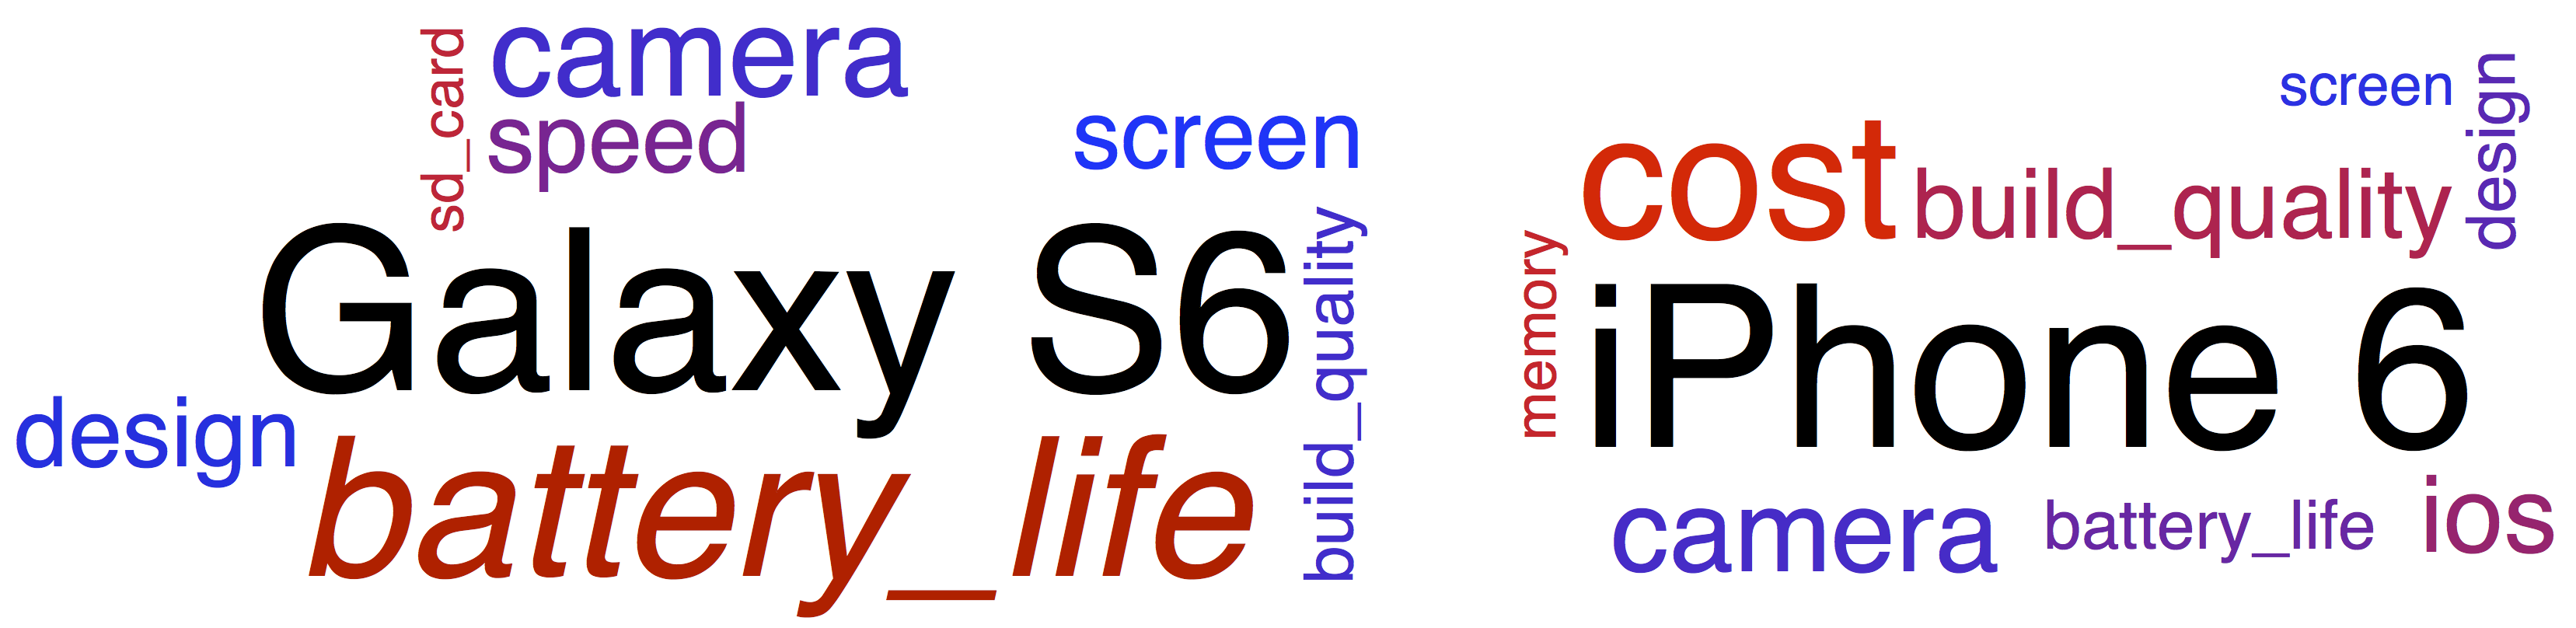
\includegraphics[width=\columnwidth]{productCloud.png}
\end{center}
\caption{Word-cloud visualizations of how \texttt{(aspect, sentiment)} tuples across multiple products can be summarized. The size of the aspect is proportional to the frequency, while the colors represent sentiment, interpolated between blue (positive) and red (negative). }
\label{productFig}
\end{figure}

We next performed a qualitative evaluation of a potential application of our model: aggregated aspect-specific reviews. We considered reviews of two popular cell phones, the Samsung Galaxy S6 and the Apple iPhone 6, and provided a visualization of the averaged sentiment in Fig. \ref{productFig}, where the word size reflects the frequency of occurrences of that aspect in the reviews, and the colors represented the sentiment associated with it. 

The visualization in Fig. \ref{productFig} shows that the single most talked about aspect of the Galaxy S6 is its battery life, which also happens to be rated rather negatively. In contrast, "battery life" is less mentioned in the reviews of the iPhone 6 and is rated more positively. The biggest complaint of the iPhone 6 seems to be its cost, while that was mentioned a lot less in the reviews of the Galaxy S6 (below the threshold we set for our visualization). Thus, a consumer who might be deciding between the Galaxy S6 and the iPhone 6 would be able to weigh specific features (e.g. how important is battery life for this consumer) very quickly and accurately without having to read through multiple (and often lengthy) reviews.

One other source of aspect-specific reviews are specialized websites that offer ``expert reviews", and often offers ratings of individual (but broader) aspects. These reviews, however, are based on the opinion of one person or a small team of reviewers and are inherently biased. As a comparison, we examined reviews of the same two products on cnet.com, a website that specializes in electronics product reviews. The Galaxy S6 on cnet.com received an 8 (out of 10) on Battery life, 9 on Features, 9 on Design, 8 on Camera and 9 on Performance. The editor's rating was 8.9 overall (4.5 stars), and the average user review was about 3 stars from 41 user reviews. The iPhone 6 was given a 9/10 for each of Design, Features and Performance, and an overall editor rating of 9/10, or 4.5 stars, compared with about 4 stars from 43 user reviews. Interestingly, the cnet editor's overall ratings for the Galaxy S6 seemed to diverge with the average cnet user rating (4.5 vs. 3). Moreover, the cnet editor's high rating of the Galaxy's battery life seemed at odds with the general sentiment of the average Amazon user. This suggests some discrepancy between ``expert reviewers" and ``average reviewers" (i.e. the consumers). This application also suggests that leveraging the "wisdom of the crowd" might provide more accurate reviews of a product than reviews from individual ``experts".

\subsubsection{Error Analysis}
Below we describe some of the bigger errors in our approach.

One common problem with the discovered aspects is the vagueness of some of the aspects. For instance, \texttt{sd\_card} was a fairly frequent aspect that came up for a Galaxy S6 smartphone. Upon further inspection of the reviews, we found that \texttt{sd\_card} referred to the \textit{lack} of a microSD card slot which prior iterations of the Galaxy had.

We also noticed that a sentence classifier using CNNs may be inadequate in capturing the subtlety in sentiment expressed in product reviews (as compared to hierarchical models such as [7]). For example, phrases like ``my old laptop was better" seems scored positively on our model, but actually reflects negative sentiment with respect to the product being discussed.

\section{Future Work}
We would like to explore a semi-supervised or active learning approach as an alternative to labeling large quantities of examples after pre-labeling for training a fully supervised model. In this case, we will have to label significantly less examples which will in turn save us time and cost. The proposed method as a whole would also be more cost efficient and scalable.

We also intend to develop our work in this report as a web application or service to provide consumers with aggregated aspect-specific sentiments of products in an intuitive and concise fashion.

\section{Conclusion}

Our model provides a cost and time efficient way of extracting high-quality aspect-level sentiment from the immense amount of unlabeled customer reviews available on online retailers such as Amazon. A lot of work is still required to productize a technology as described in this report, however, the results we have observed so far with our models have been greatly optimistic.  We believe that such an application that extracts and aggregates aspect-specific reviews across the Web would be a huge boon to both the electronic commerce industry and consumers alike.

\subsubsection*{Acknowledgments}

We would like to thank Richard Socher and the teaching assistants of CS224D for all their help and the Stanford Deep Social Learning Lab for providing computing resources.

\subsubsection*{References} % chronological. Use APA

\small{

%Word2Vec papers
[1] Mikolov, T. \& Chen, K. \& Corrado, G. \& Dean, J. (2013). Efficient Estimation of Word Representations in Vector Space. In Proceedings of Workshop at ICLR, 2013.

[2] Mikolov, T. \& Chen, K. \& Corrado, G. \& Dean, J. (2013). Distributed Representations of Words and Phrases and their Compositionality. In Proceedings of NIPS, 2013.

[3] Titov, I., \& McDonald, R. T. (2008). A Joint Model of Text and Aspect Ratings for Sentiment Summarization. In {\it ACL} (Vol. 8, pp. 308-316).

[4] Brody, S., \& Elhadad, N. (2010). An unsupervised aspect-sentiment model for online reviews. In {\it Human Language Technologies: The 2010 Annual Conference of the North American Chapter of the Association for Computational Linguistics} (pp. 804-812). Association for Computational Linguistics.

[5] Jo, Y., \& Oh, A. H. (2011). Aspect and sentiment unification model for online review analysis. In Proceedings of the fourth ACM international conference on Web search and data mining (pp. 815-824). ACM.


[6] Engonopoulos, N., Lazaridou, A., Paliouras, G., \& Chandrinos, K. (2011). ELS: a word-level method for entity-level sentiment analysis. In {\it Proceedings of the International Conference on Web Intelligence, Mining and Semantics}


[7] Moilanen, K., \& Pulman, S. (2009). Multi-entity Sentiment Scoring. In {\it Recent Advances in NLP} (pp. 258-263).


[8] Lakkaraju, H., Socher, R, \& Manning, C. (2014). Aspect Specific Sentiment Analysis using Hierarchical Deep Learning. {\it NIPS Workshop on Deep Learning and Representation Learning}

[9] Socher, R., Perelygin, A., Wu, J. Y., Chuang, J., Manning, C. D., Ng, A. Y., \& Potts, C. (2013). Recursive deep models for semantic compositionality over a sentiment treebank. In {\it Proceedings of the conference on Empirical Methods in Natural Language Processing (EMNLP)} (Vol. 1631, p. 1642).

[10] Kim, Y. (2014). Convolutional neural networks for sentence classification. EMNLP.

[11] McAuley, J., Targett, C., Shi, J., \& van den Hengel, A. (2015). Image-based recommendations on styles and substitutes. {\it ACM Special Interest Group on Information Retrieval (SIGIR)}

[12] Bird, S, Loper, E. and Klein, E. (2009). Natural Language Processing with Python. O'Reilly Media Inc.

[13] Hu, M., \& Liu, B. (2004). Mining and summarizing customer reviews. In Proceedings of the tenth ACM SIGKDD international conference on Knowledge discovery and data mining (pp. 168-177). ACM.


[14] Hinton, G., Srivastava, N., Krizhevsky, A., Sutskever, I., Salakhutdinov, R. (2012). Improving neural networks by preventing co-adaptation of feature detectors. CoRR, abs/1207.0580.






%% this paper isn't that relevant. it's an evaluation system.
%[2] Ward, C. B., Choi, Y., Skiena, S., \& Xavier, E. C. (2011). Empath: A framework for evaluating entity-level sentiment analysis. In {\it Emerging Technologies for a Smarter World (CEWIT), 2011 8th International Conference \& Expo}. (pp. 1-6). IEEE.


%
%Wang, H., Lu, Y., & Zhai, C. (2010, July). Latent aspect rating analysis on review text data: a rating regression approach. In Proceedings of the 16th ACM SIGKDD international conference on Knowledge discovery and data mining (pp. 783-792). ACM.
%
%Yatani, K., Novati, M., Trusty, A., & Truong, K. N. (2011, May). Review spotlight: a user interface for summarizing user-generated reviews using adjective-noun word pairs. In Proceedings of the SIGCHI Conference on Human Factors in Computing Systems (pp. 1541-1550). ACM.



}

\end{document}
